% !TeX program = pdflatex
\documentclass[tikz,border=8pt]{standalone}
\usepackage{tikz}
\usetikzlibrary{calc,angles,quotes,positioning}
\definecolor{FigureBlue}{HTML}{2563EB}
\definecolor{FigureOrange}{HTML}{EA580C}
\begin{document}
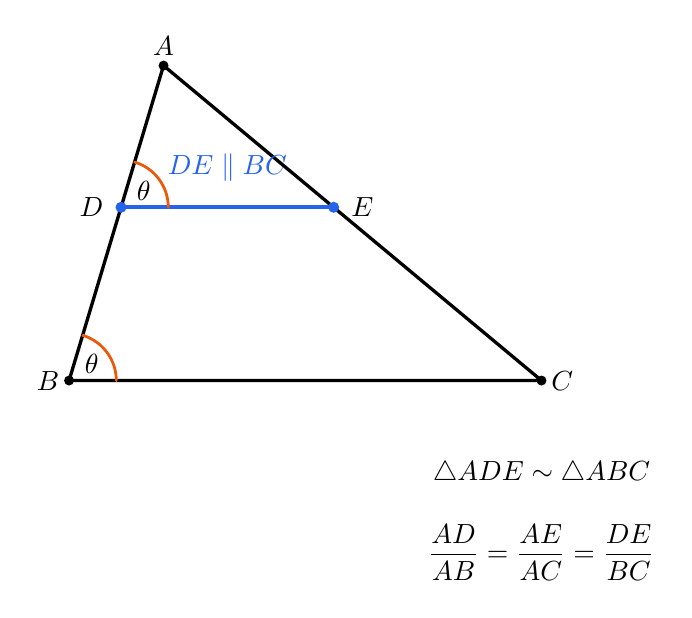
\begin{tikzpicture}[line cap=round,line join=round]
  \coordinate (A) at (1.2,4);
  \coordinate (B) at (0,0);
  \coordinate (C) at (6,0);
  \coordinate (D) at ($(A)!.45!(B)$);
  \coordinate (E) at ($(A)!.45!(C)$);

  \draw[line width=1.2pt] (A)--(B)--(C)--cycle;
  \draw[FigureBlue,line width=1.5pt] (D)--(E);
  \pic[draw=FigureOrange,line width=1pt,angle radius=6mm,"$\theta$"] {angle=E--D--A};
  \pic[draw=FigureOrange,line width=1pt,angle radius=6mm,"$\theta$"] {angle=C--B--A};

  \fill (A) circle (1.8pt) (B) circle (1.8pt) (C) circle (1.8pt);
  \fill[FigureBlue] (D) circle (2pt) (E) circle (2pt);
  \node[above] at (A) {$A$};
  \node[left] at (B) {$B$};
  \node[right] at (C) {$C$};
  \node[left=1mm] at (D) {$D$};
  \node[right=1mm] at (E) {$E$};
  \node[above=2mm,FigureBlue] at ($(D)!.5!(E)$) {$DE\parallel BC$};
  \node[below=9mm of C.west,anchor=north] {$\triangle ADE\sim\triangle ABC$};
  \node[below=17mm of C.west,anchor=north] {$\displaystyle\frac{AD}{AB}=\frac{AE}{AC}=\frac{DE}{BC}$};
\end{tikzpicture}
\end{document}
